\documentclass{article}
%%%%%%%%%%%%%%%%%%%%%%%%%%%%%%%%%%%%%%%%%
% Lachaise Assignment
% Structure Specification File
% Version 1.0 (26/6/2018)
%
% This template originates from:
% http://www.LaTeXTemplates.com
%
% Authors:
% Marion Lachaise & François Févotte
% Vel (vel@LaTeXTemplates.com)
%
% License:
% CC BY-NC-SA 3.0 (http://creativecommons.org/licenses/by-nc-sa/3.0/)
% 
%%%%%%%%%%%%%%%%%%%%%%%%%%%%%%%%%%%%%%%%%

%----------------------------------------------------------------------------------------
%	PACKAGES AND OTHER DOCUMENT CONFIGURATIONS
%----------------------------------------------------------------------------------------

\usepackage{amsmath,amsfonts,stmaryrd,amssymb,subcaption} % Math packages

\usepackage{enumerate} % Custom item numbers for enumerations

\usepackage[ruled]{algorithm2e} % Algorithms

\usepackage[framemethod=tikz]{mdframed} % Allows defining custom boxed/framed environments

\usepackage{listings} % File listings, with syntax highlighting
\lstset{
	basicstyle=\ttfamily, % Typeset listings in monospace font
}

\usepackage{hyperref}

%----------------------------------------------------------------------------------------
%	DOCUMENT MARGINS
%----------------------------------------------------------------------------------------

\usepackage{geometry} % Required for adjusting page dimensions and margins

\geometry{
	paper=a4paper, % Paper size, change to letterpaper for US letter size
	top=2.5cm, % Top margin
	bottom=2.5cm, % Bottom margin
	left=2.5cm, % Left margin
	right=2.5cm, % Right margin
	headheight=14pt, % Header height
	footskip=1.5cm, % Space from the bottom margin to the baseline of the footer
	headsep=1.2cm, % Space from the top margin to the baseline of the header
	%showframe, % Uncomment to show how the type block is set on the page
}

%----------------------------------------------------------------------------------------
%	FONTS
%----------------------------------------------------------------------------------------

\usepackage[utf8]{inputenc} % Required for inputting international characters
\usepackage[T1]{fontenc} % Output font encoding for international characters

\usepackage{XCharter} % Use the XCharter fonts

%----------------------------------------------------------------------------------------
%	COMMAND LINE ENVIRONMENT
%----------------------------------------------------------------------------------------

% Usage:
% \begin{commandline}
%	\begin{verbatim}
%		$ ls
%		
%		Applications	Desktop	...
%	\end{verbatim}
% \end{commandline}

\mdfdefinestyle{commandline}{
	leftmargin=10pt,
	rightmargin=10pt,
	innerleftmargin=15pt,
	middlelinecolor=black!50!white,
	middlelinewidth=2pt,
	frametitlerule=false,
	backgroundcolor=black!5!white,
	frametitle={Command Line},
	frametitlefont={\normalfont\sffamily\color{white}\hspace{-1em}},
	frametitlebackgroundcolor=black!50!white,
	nobreak,
}

% Define a custom environment for command-line snapshots
\newenvironment{commandline}{
	\medskip
	\begin{mdframed}[style=commandline]
}{
	\end{mdframed}
	\medskip
}

%----------------------------------------------------------------------------------------
%	FILE CONTENTS ENVIRONMENT
%----------------------------------------------------------------------------------------

% Usage:
% \begin{file}[optional filename, defaults to "File"]
%	File contents, for example, with a listings environment
% \end{file}

\mdfdefinestyle{file}{
	innertopmargin=1.6\baselineskip,
	innerbottommargin=0.8\baselineskip,
	topline=false, bottomline=false,
	leftline=false, rightline=false,
	leftmargin=2cm,
	rightmargin=2cm,
	singleextra={%
		\draw[fill=black!10!white](P)++(0,-1.2em)rectangle(P-|O);
		\node[anchor=north west]
		at(P-|O){\ttfamily\mdfilename};
		%
		\def\l{3em}
		\draw(O-|P)++(-\l,0)--++(\l,\l)--(P)--(P-|O)--(O)--cycle;
		\draw(O-|P)++(-\l,0)--++(0,\l)--++(\l,0);
	},
	nobreak,
}

% Define a custom environment for file contents
\newenvironment{file}[1][File]{ % Set the default filename to "File"
	\medskip
	\newcommand{\mdfilename}{#1}
	\begin{mdframed}[style=file]
}{
	\end{mdframed}
	\medskip
}

%----------------------------------------------------------------------------------------
%	NUMBERED QUESTIONS ENVIRONMENT
%----------------------------------------------------------------------------------------

% Usage:
% \begin{question}[optional title]
%	Question contents
% \end{question}

\mdfdefinestyle{question}{
	innertopmargin=1.2\baselineskip,
	innerbottommargin=0.8\baselineskip,
	roundcorner=5pt,
	nobreak,
	singleextra={%
		\draw(P-|O)node[xshift=1em,anchor=west,fill=white,draw,rounded corners=5pt]{%
		Question \theQuestion\questionTitle};
	},
}

\newcounter{Question} % Stores the current question number that gets iterated with each new question

% Define a custom environment for numbered questions
\newenvironment{question}[1][\unskip]{
	\bigskip
	\stepcounter{Question}
	\newcommand{\questionTitle}{~#1}
	\begin{mdframed}[style=question]
}{
	\end{mdframed}
	\medskip
}

%----------------------------------------------------------------------------------------
%	WARNING TEXT ENVIRONMENT
%----------------------------------------------------------------------------------------

% Usage:
% \begin{warn}[optional title, defaults to "Warning:"]
%	Contents
% \end{warn}

\mdfdefinestyle{warning}{
	topline=false, bottomline=false,
	leftline=false, rightline=false,
	nobreak,
	singleextra={%
		\draw(P-|O)++(-0.5em,0)node(tmp1){};
		\draw(P-|O)++(0.5em,0)node(tmp2){};
		\fill[black,rotate around={45:(P-|O)}](tmp1)rectangle(tmp2);
		\node at(P-|O){\color{white}\scriptsize\bf !};
		\draw[very thick](P-|O)++(0,-1em)--(O);%--(O-|P);
	}
}

% Define a custom environment for warning text
\newenvironment{warn}[1][Warning:]{ % Set the default warning to "Warning:"
	\medskip
	\begin{mdframed}[style=warning]
		\noindent{\textbf{#1}}
}{
	\end{mdframed}
}

%----------------------------------------------------------------------------------------
%	INFORMATION ENVIRONMENT
%----------------------------------------------------------------------------------------

% Usage:
% \begin{info}[optional title, defaults to "Info:"]
% 	contents
% 	\end{info}

\mdfdefinestyle{info}{%
	topline=false, bottomline=false,
	leftline=false, rightline=false,
	nobreak,
	singleextra={%
		\fill[black](P-|O)circle[radius=0.4em];
		\node at(P-|O){\color{white}\scriptsize\bf i};
		\draw[very thick](P-|O)++(0,-0.8em)--(O);%--(O-|P);
	}
}

% Define a custom environment for information
\newenvironment{info}[1][Info:]{ % Set the default title to "Info:"
	\medskip
	\begin{mdframed}[style=info]
		\noindent{\textbf{#1}}
}{
	\end{mdframed}
}
 % Include the file specifying the document structure and custom commands
\usepackage{subcaption}

\title{SI 649: Communication Visualization Project \\ Interactive Blog Post} % Title of the assignment

\author{Mingliang Duanmu\\ \texttt{duanmuml@umich.edu}} % Author name and email address

\date{\today} % University, school and/or department name(s) and a date

\begin{document}

\maketitle % Print the title

\section{Learning Objectives}

The viewer will be able to:
\begin{itemize}
    \item \textbf{Conclude} the diseases with highest mortality in Red Lake County and the trend of mortality during the past 30 years.
    \item \textbf{Contrast} the unemployment rate, average household income, and poverty rate of Red Lake County to the national and state-level data.
    \item \textbf{Observe} the difference between educational resources within the state of Minnesota, and across different states in the US.
\end{itemize}

\section{Design Process}

\subsection*{Idea}

Most of my ideas of building the visualizations are based on the aspects mentioned by the author in the article "I called this place ‘America’s worst place to live.’ Then I went there". The static version of my visualization focuses on comparisons of Red Lake County statistics against national average or counties within the same state. I apply various methods of encoding, representation and annotation to make it quick for readers to notice the contrast. I also go a little beyond to display extra aspects of Red Lake County that add to a more complete impression of the place for readers.

\subsection*{Data}

I search extensively online to find useful and credible datasets for my visualizations. The data sources include Kaggle (the mortality data, public school data), USDA (natural amenity), U.S. Census Bureau (poverty and household income), U.S. Bureau of Labor Statistics (unemployment rate). \\
\noindent
Based on the date of the article, all my visualizations are based on the data before 2015. I do some data cleaning and filtering on the raw data to kick out wrong values and useless information, as well as reorganizing structures of tables to make them more suitable to Altair grammar.

\subsection*{Tool}

I use a combination of Altair and Streamlit for my interactive visualizations. Streamlit is an easy-to-use, lightweight tool to deploy blog sites using Python. The interaction widgets like select boxes, sliders, checkboxes and radio buttons can be well combined with parameters of Altair graphs to provide convenient interactions with readers. As a person used to programming-based tools, Altair has more freedom of customizing all the parameters of a graph, together with versatility to add interface interactions and organize multiple subplots. I give up using Tableau in this interactive due to high learning cost.

\subsection*{Visualizations}

\subsubsection*{Line plot for unemployment rate}

Since the author claims that Red Lake County's unemployment rate is well below national level, I decide to use a line plot to compare it with the national data. Unluckily the unemployment rate I find only applies to each state since county-level data are missing for many states. \\
\begin{figure}[htbp]
    \centering
    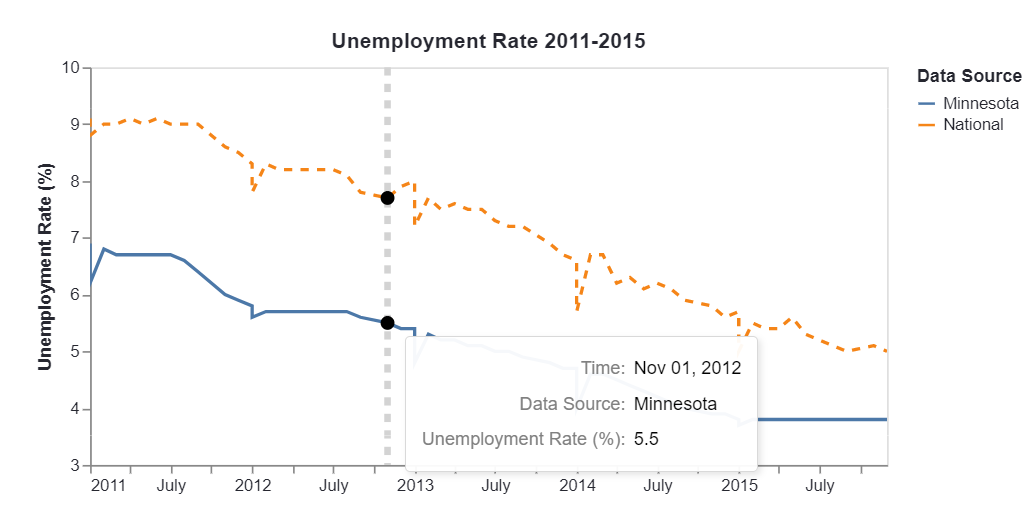
\includegraphics[scale=0.9]{v1.png}
    \caption{Line Plot for unemployment rate}
\end{figure} \\
Interactions: \\
\begin{itemize}
    \item I add zooming to both x and y axis to allow users to view local values and trends easily.
    \item Similar as homework, I add a grey vertical line and two black dots when mouse is hovering on the data points, so that reader can easily compare the value of national and Red Lake's unemployment rate at the same time point.
\end{itemize}
What I dislike about this plot is that the information is not rich, which is due to the limitation of data from the source. The graph is already expressive so it does not require extra interaction to make it more efficient.

\newpage
\subsubsection*{Dual scatter plots for average household income, and poverty rate}
\noindent
Since the author mentions that Red Lake County does not rank low on economic metrics like household income and poverty rate, I decide to use scatter plots to display such two metrics in both national scale and state scale. \\
\noindent
For the scatter plot, I try different encodings of three features on both axises and size/color, to minimize influence on the size of graph by outliers. Finally I came up with the dual plots in Figure 2.
\begin{figure}[htbp]
    \centering
    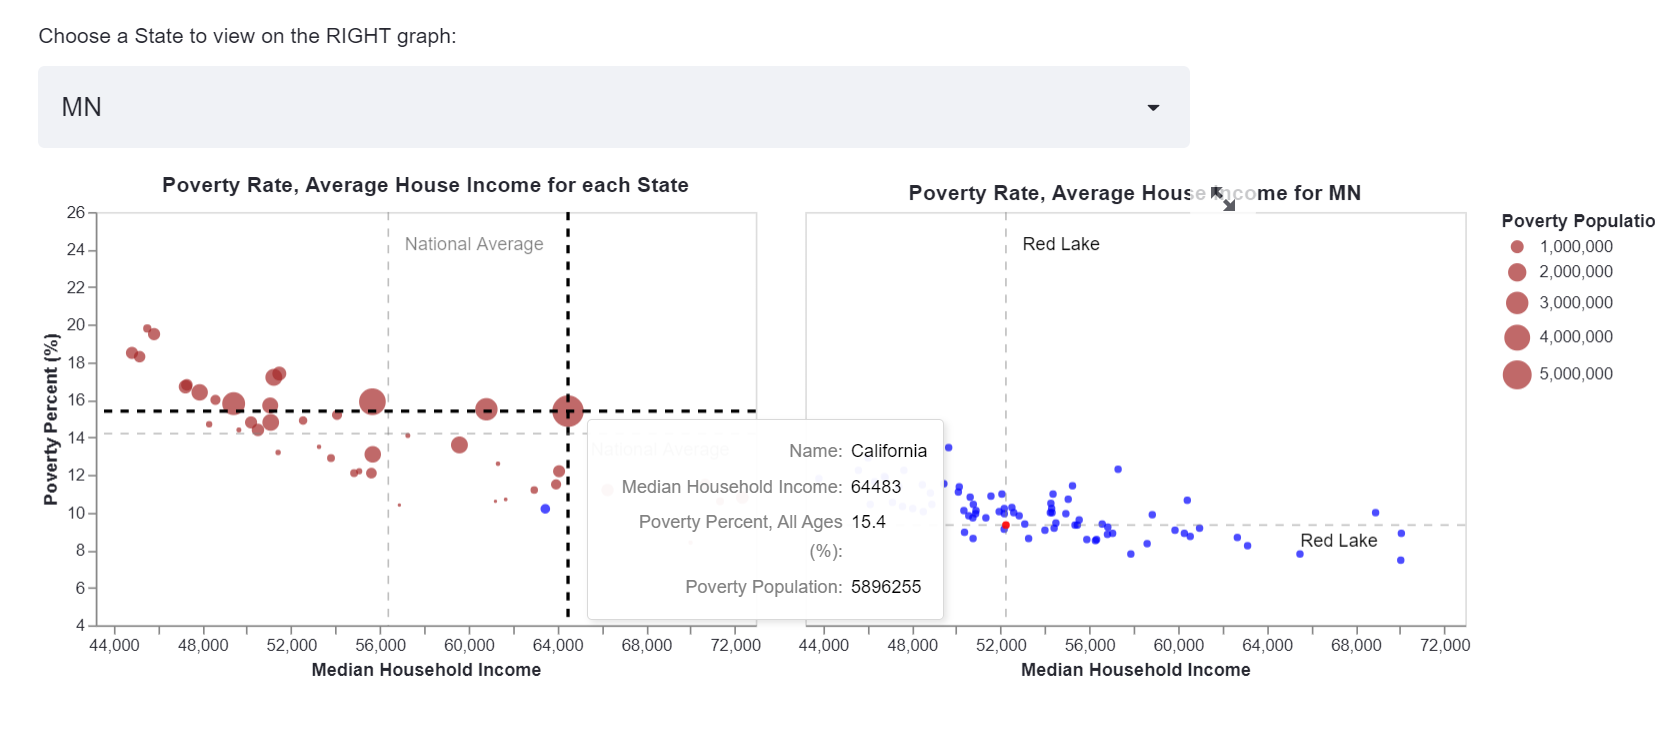
\includegraphics[scale=0.55]{v2.png}
    \caption{Dual Scatter Plot for poverty rate, poverty population, household income}
\end{figure} \\
\noindent
The position of Minnesota is marked with blue color on the left plot. The grey dash lines indicate average value of each dimension on the left plot and the value of Red Lake County on the right plot. Both plots share the same y-axis. \\
\noindent
I tried log scale on the x-axis but I think it prevents readers from knowing the real numbers and it makes deviation from average value look smaller for large data. Also, The distance between dots are narrower. \\
Interactions:
\begin{itemize}
    \item I add zooming to x axis to allow users to view local values among a series of scatter points easily.
    \item When clicking on the points on the left plot, a vertical and a horizontal black dash line help readers read the exact values on both axises.
    \item The tooltip displays the state name and all three features on mouse hovering.
    \item Readers can use the selection menu to view data of different states in the right plot, at the same time comparing it to national data. The default of selection is MN. 
    \item The point indicating Red Lake County is marked red and always displayed so readers can even know the position of Red Lake County in other states across the country. 
\end{itemize}

\newpage
\subsubsection*{Bar and scatter plot for public school statistics}

As the author mentions education as an important thing in Red Lake County, I decide to contrast the level of educational resources of the county with other counties in Minnesota and the average domestic statistics. I only include data of public schools because there is no private ones in Red Lake. \\
\noindent
I created two calculation fields, one is student per teacher and the other is enrollment rate. A small number of students assigned to each teacher means the educational resources is more abundant. The enrollment rate, which equals to enrollment number divided by the right-age population, is a good indicator of the willingness of pursuing education. \\
\begin{figure}[htbp]
    \centering
    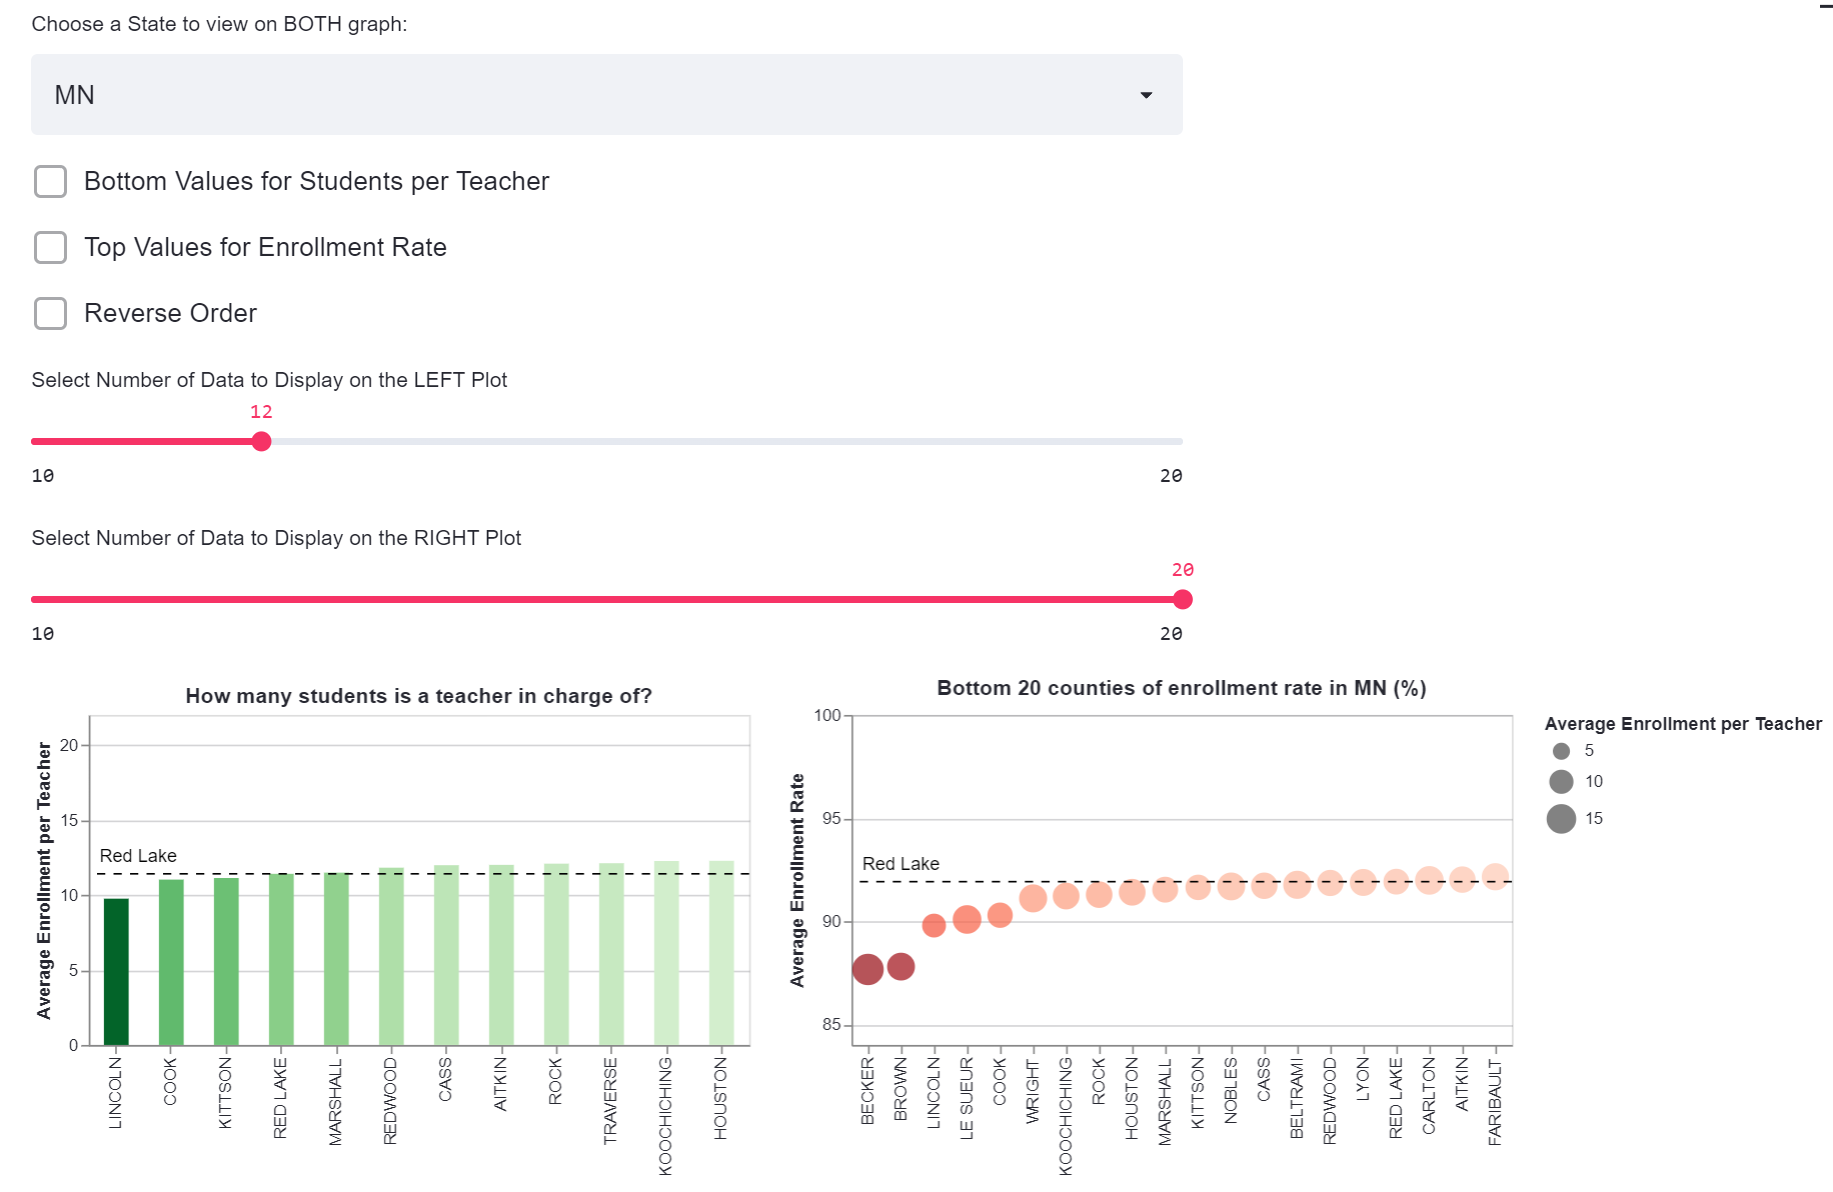
\includegraphics[scale=0.5]{v3.png}
    \caption{Bar chart and dot chart for educational resources}
\end{figure} \\
Interactions:
\begin{itemize}
    \item Readers can use the selection menu to explore educational resources regarding the two aspects for different states across the country. The default of selection is MN.
    \item Using the checkboxes, readers are able to switch between top/bottom values for both metrics, as well as changing the display according to ascending/descending order.
    \item The sliders allow readers to customize the number of top/bottom values they want to display on both plots. A range between 10 and 20 is available for choice.
    \item The tooltip displays the exact numerical value on mouse hovering.
    \item The value of Red Lake County is marked using a horizontal dash line and always displayed so readers can even know the position of Red Lake County in other states across the country. 
\end{itemize}
\noindent
What I dislike about the graph is that the size encoding on the right graph is not distinct enough, since the range of average enrollment per teacher is narrow. \\
\noindent
Previously I tried to include the top/bottom 5 values for the left plot in Tableau, but I found there is no necessity and does not add to expressiveness. \\


\newpage
\subsubsection*{Line/heatmap and scatter plot for mortality}

In this graph, I go a little beyond the content of the article, but I think health is also an important evaluation of whether a place is suitable to live in. I want to see the major diseases causing death and if the health condition improves with time in such a "worst place to live". \\
\noindent
I use a line chart, a scatter plot and a heatmap to display the top 5 mortal diseases in Red Lake and the change of mortality with time. On the heatmap, the mortality rates of the most and least recent time are highlighted to inform readers the change during the period. I also make a comparison with national value on the top 5 diseases in Red Lake in terms of the percentage of change in mortality from 1980 to 2014. \\
\begin{figure}[htbp]
    \begin{subfigure}{.5\textwidth}
        \centering
        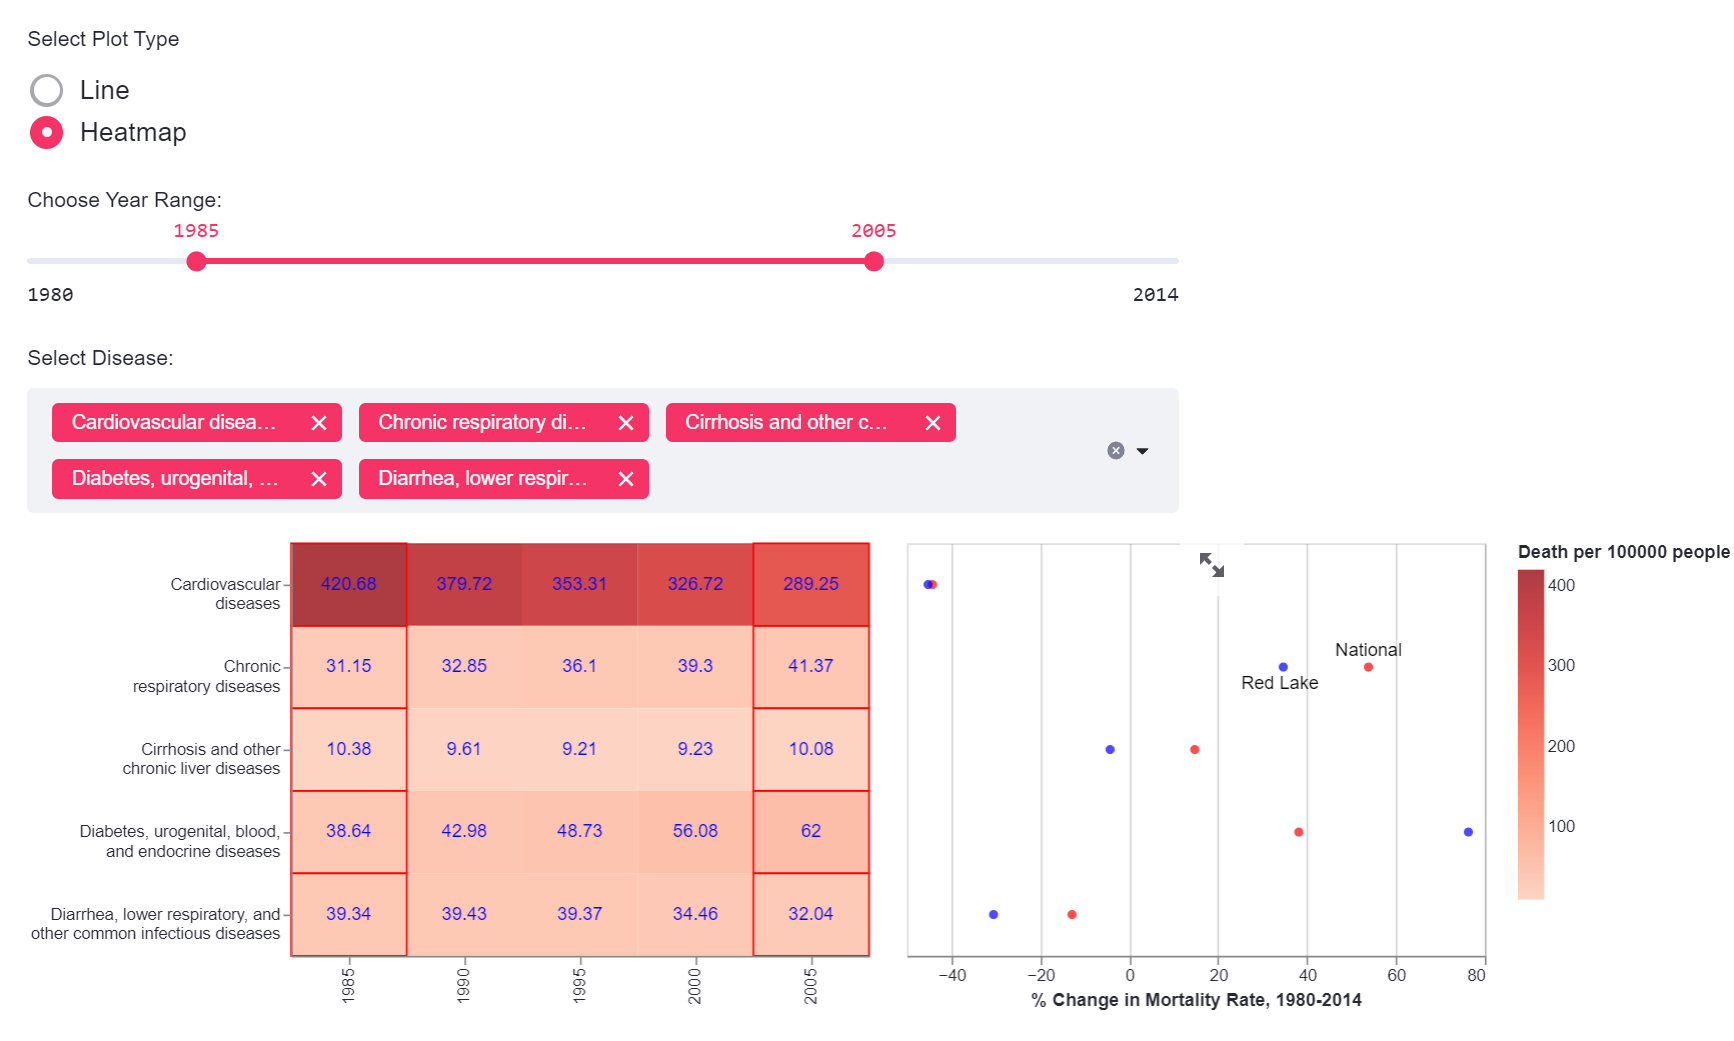
\includegraphics[width=\linewidth]{v4_1.png}
        \caption{Heatmap}
    \end{subfigure}
    \begin{subfigure}{.5\textwidth}
        \centering
        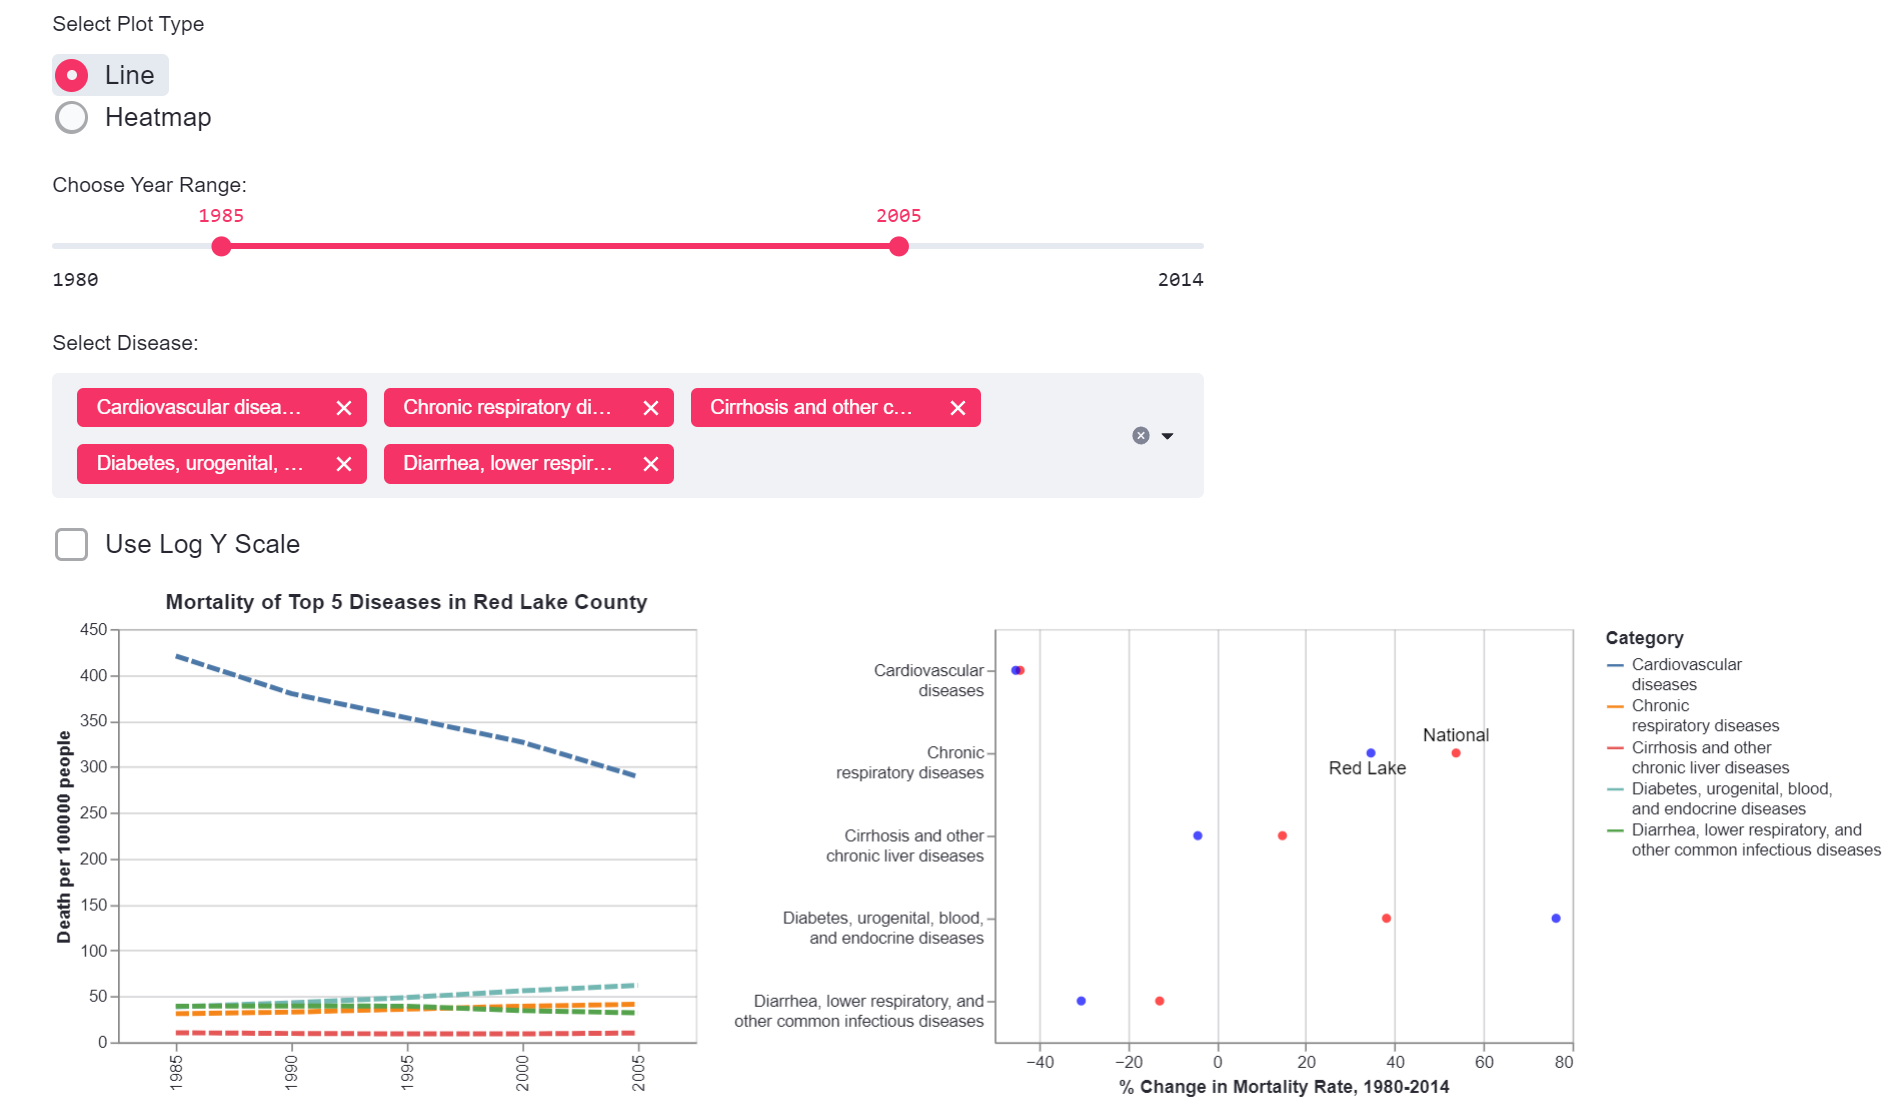
\includegraphics[width=\linewidth]{v4_2.png}
        \caption{Line}
    \end{subfigure}
    \caption{Heatmap/Line plot for top 5 mortal diseases in Red Lake}
\end{figure} \\
Interactions:
\begin{itemize}
    \item Readers can choose either the heatmap or line plot to display the trend of diseases in the past 35 years using the radio button.
    \item For the line plot, readers can use the checkbox to change y values to log scale for comparisons between diseases.
    \item Readers can customize the range of timeline for both the heatmap and line plot using a double ended slider.
    \item Readers can choose different subsets of diseases to display on both plots using the multiple selection box. All five diseases are shown by default.
\end{itemize}
\noindent
As the dataset provides min/max values for each year's data, I planned to embed those boundaries into the line chart and the scatter plot, however it appeared too crowdy on the graphs and it is enough for readers to figure out the trends and features of data without knowing the specific ranges.


\newpage
\section{Final Design}

\begin{itemize}
    \item \textbf{Perception} \\
    Color: \\
    I use different color encodings in my visualizations that conform to reader's perception habits. I use green color to encode data containing positive aspects like high educational resources. In contrast, red color represents negative data like mortality and bad enrollment rate. For example, lighter red represents less fatality for a disease (Figure 4). In the scatter plot, there is a color consistency between the highlighted data point on the left graph and dots in the right graph (Figure 2). \\ 
    \noindent
    Cognition: \\
    In the scatter plot, I create a pop-out effect using a contrast color to identify the point we want to observe (Figure 2). For multiple lines crossing each other in one chart (Figure 4), color encoding is a good way to reinforce Gestalt Principle of continuity for readers.
    \item \textbf{Design} \\
    Data Ink: \\
    I pay careful attention to maximize the data ink ratio in my visualizations. For time-oriented axis (Figure 1, 4) and categorical variable axis (Figure 4), I erase the grid lines in those dimensions and only leave the grid lines for numerical variables in the purpose of precise reference. Also for the scatter plot (Figure 2), I change the range of both axis to the data range to avoid leaving much blank and make data points sparse on the plot. \\
    \noindent
    Graphic Integrity: \\ 
    All the data in my visualizations are compared and drawn in the same scale, so the lie factors of all graphs are one. I avoid using a logarithm scale on population data to make deviations from mean value different for small and great values, as log scale makes distance between great values narrower. I make necessary annotations for average values (Figure 2), heatmap cells (Figure 4), and customized color encodings (Figure 4), through bold black font and dash grey lines. All my plots are in 2D, carrying at most three dimensions of data in total, with the extra dimension encoded with color or size. 
    \item \textbf{Interaction} \\
    Filter: \\
    I use filters on time, variables and items to display on the last two plots. A double ended slider on time interval allows user to choose data within any time period to display, and a multiple selection box makes readers focus only on the categories they are interested in. \\
    Explore: \\
    For the second and third plot, I offer a dropdown menu for readers to choose different states' data to display. Although the topic is about Red Lake County, the readers can explore the same metrics on different places across the nation, which gives them a broader picture of national level and makes a fairer context for Red Lake. Also, the slider and checkboxes on the number of top/bottom counties to display satisfies readers' curiosity in the counties doing good/bad on certain metric, as well as the large gap between top and bottom performances. \\
    Encoding: \\
    For the mortality plot, I provide two encoding options on the same data for readers to choose from, line plot and heatmap. Each encoding has its benefit in conveying information according to reader preference: line plot focuses on the trend of mortality of each disease along the timeline and provides parallel comparison between different diseases, while heatmap shows the severity of disease of any time point in a straightforward color encoding, and the text labels and highlights make the detail values clearer.
\end{itemize}

\newpage

\section{Evaluation Method}

To ensure the readers can fulfill my learning object described in the first section, a simple way is to ask a few domain questions about the information we want them to take away, for example:
\begin{itemize}
    \item What diseases have a high death rate for Red Lake County and are there any trends of decrease/increase in mortality with the time? Which diseases did Red Lake County effectively protect against compared to national average after 35 years?
    \item Where is the position of Red Lake County's poverty situation and household income if we put it in a national scale? Does Red Lake County defeat half of the counties in California in terms of poverty rate? Can you give an example of state with a lower average income and higher poverty rate than Red Lake County?
    \item What is good about Red Lake County and what is the problem we still need to solve in terms of public education? How big is the difference between top and bottom counties within a certain state in terms of education resources?
\end{itemize}

\noindent
Also a usability test should be done to collect feedback from different users, depending on their social roles, ages, and degree of mastery on reading electronic visualizations. The usability test should be conducted using the control variate method, which means we may only change one factor each time, for example, color encoding, sequence of graph, or annotation font size, to figure out their actual influence on completing the learning objectives.

\end{document}
